\chapter{Background}

\section{Graph Theory}

Before we begin discussing different visualization techniques, it is important to understand the data behind the visualization. As we are not limiting ourselves to a specific application domain, the key is to understand the structure of the data. Simply speaking we are dealing with graph or network data, but as there are multiple terms and terminologies used we want to give a short summary. 

In general, a graph consists of vertices and edges \cite{diestel_graph_2017}. In the context of this thesis we also use the terms nodes for vertices, links for edges and network for graph interchangeably. Furthermore, edges in a graph can either be directed or undirected. Directed edges differentiate between source and target node where undirected edges do not. Additionally, we also distinguish between weighted and unweighted edges. Weighted edges have any sort of numerical comparable attribute. This can be used for instance to describe how strong the relation between nodes is. Figure \ref{fig:simple_weighted_directed_network} shows a directed and weighted graph.

A specialized version of a graph is called tree. It is defined as an acyclic graph where all subcomponents of the graph are connected \cite{diestel_graph_2017}. One node of the tree can be picked as a root node which is usually drawn on the top. Nodes with only one link are called leaf nodes and drawn on the bottom, see Figure \ref{fig:simple_tree}.\\
In addition, tree nodes also have a height and depth. The height is defined by the largest number of edges between the root node and a leaf node. The height of the root node is the height of the tree itself. The dept of the node is the number of edges along the path to the root node. Note that a tree is able to encode hierarchical relationships between nodes. In the thesis we use the term 'hierarchical level' for depth and terminologies like 'leaf1 is a direct child of node1' or 'node1 is the parent (node) of leaf1' based on Figure \ref{fig:simple_tree}.

In addition to the basic graph structures, which are often not sufficient for specific datasets, there are extended forms of graph models \cite{bertault_algorithm_1999}. 
%higraph, clustered graph, compound graph
For the context of this thesis, clustered graphs are especially interesting. A clustered graph is defined by a recursive structure where each node can be new graph for itself \cite{eades_multilevel_1997}.\\ 
%Another would be a compound graph. a set of different elements such as vertices or edges and therefore 
%compound graph (master thesis), 
Furthermore, multivariate networks \cite{kerren_introduction_2014} combines the data type of network with multidimensional datasets. Each node and edge can have numerous additional attributes these can be numerical, ordinal or categorical.

\begin{figure}[h]
    \centering
    \begin{subfigure}[b]{0.45\columnwidth}
        \centering
        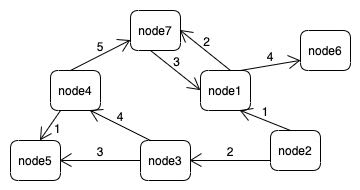
\includegraphics[width=\textwidth]{graphics/weightedDirectedNetwork.jpg}
        \subcaption{Weighted and directed graph.}
        \label{fig:simple_weighted_directed_network}
    \end{subfigure}
    \begin{subfigure}[b]{0.54\columnwidth}
        \centering
        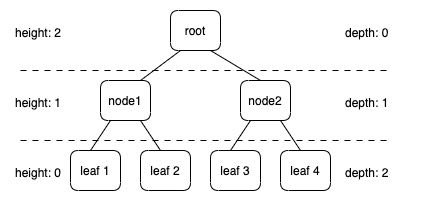
\includegraphics[width=\textwidth]{graphics/basicTree.jpg}
        \subcaption{Tree with a height of 2.}
        \label{fig:simple_tree}
    \end{subfigure}
    
    \caption[Optional caption for the figure list (often used to abbreviate long captions)]{Simple visualizations of graph data structures} % Remove the [...] argument if the original caption should be used in the figure list.
    \label{fig:intro} 
  \end{figure}

In conclusion, the most basic graph or network would be a simple unweighted and undirected set of nodes and links without any hierarchical relationship. To be able to represent different types of relationships in our data their exists different extensions. 

\subsection{Graph Drawing}

As graph drawing is a subarea of information visualization, common knowledge from this research area can be applied here as well. With Shneiderman's visual information seeking mantra “Overview first, zoom and filter, then details-on-demand” being one of the most famous \cite{shneiderman_eyes_1996}. Additionally, the Gestalt Principles can also be used in graph drawing as Kobourov et al.
\cite{kobourov_gestalt_2015} shows us. They can be used to produce more aesthetically pleasing visualizations by defining drawing conventions and even improve the impression of the data. Cluster affiliation of nodes can be expressed by similar colors, shapes or simply by proximity. While the form of links should be consistent without any sharp bends.

For representation node-link and space-filling concepts are the most important for the data structures used in this thesis. Space-filling visualizations usually use multiscale approaches to encode hierarchical information. Node-link graphs tend to utilize force-based or constraint-based layouts\cite{von_landesberger_visual_2011}.

Force based layout techniques work without any domain-specific knowledge, therefore provide a flexible way to determine layouts for node link graphs \cite{kobourov_spring_2012}. Only structural information about the graph relationships themselves are used. 
There are a variety of different approaches but concept is always the same. 
These systems work by providing numerous forces between nodes and links, whose job is to update the position of the nodes. Usually these forces are related to Hooke's law, a simple approach by Kamada et al. \cite{kamada_algorithm_1989} is to use repulsive forces between all nodes and attraction forces for linked nodes.
The defined forces are then processed with a given set of nodes and links for either a limited number of iterations, a fixed time, some sort of dynamic condition like the momentum of the nodes fall below a certain threshold or just infinitely.
Large graphs however are a common problem as physical force models tend to have many local minima and therefore not produce optimal results \cite{kobourov_spring_2012}.

\section{Visualization Techniques}
Papers:\\

Shneiderman\\
The Eyes Have It: A Task by Data Type Taxonomy for Information Visualizations\\
Visual Information Seeking Mantra\\
\\
Kobourov\\
Gestalt Principles in Graph Drawing\\
\\
Brath \\
3D InfoVis is Here to Stay: Deal with It\\
Warum allgemein 3D Infos Vis Vorteile hat\\
\\
Lee\\
Task Taxonomy for Graph Visualization\\
a list of tasks for graph visualization that has
enough detail and specificity to be useful to: 1) designers who
want to improve their system and 2) to evaluators who want to
compare graph visualization systems.\\
\\

\subsection{Force-directed graph drawing}
alt:\\
Fruchterman\\
Graph drawing by force-directed placement\\
\\
Kamada Kawai\\
AN ALGORITHM FOR DRAWING GENERAL UNDIRECTED GRAPHS\\
\\

aktueller:\\
Yifan Hu\\
Efficient, High-Quality Force-Directed Graph Drawing\\
Algorithmus für force Graph,  Erklärkung barnes hut etc Sehr detailliert, viel info\\
\\
Kobourov\\
Spring Embedders and Force Directed Graph Drawing Algorithms\\
Mehrere Algorithmen für Force Graph, Sehr detailliert\\
\\

\section{Network Visualization}

\subsection{Network Visualization Basics}

Kerren\\
\textbf{Introduction to Multivariate Network Visualization vorallem Chapter9: Heterogeneous Networks on Multiple Levels} \\
gute Zusammenfassung von Multilayer Network Visualization\\

West\\
Introduction to graph theory\\
\\


\section{VR Technology}

Content:
\begin{itemize}
    \item Describe the technologie stack (OpenVR, WEBXR/WEBVR, A-Frame, ThreeJS)
    \item Devices, HTC-VIVE, Oculus-Rift, Vendors
    \item Room scale vs Table vs Standing, possibilities of tracking
    \item 6 DOF vs 3 DOF (degrees of freedom)
    \item Vergleich HMD zu früheren Möglichkeiten mit "Cave" Virtual Reality
\end{itemize}

official Specs / Docs: 
\\
Desktop API:\\
https://www.khronos.org/openxr/ \\
https://github.com/ValveSoftware/openvr \\
\\
Web API:\\
   WebXR\\
https://immersiveweb.dev/ \\
https://github.com/immersive-web/webxr/blob/master/explainer.md \\
https://immersive-web.github.io/webxr/ \\
https://blog.mozvr.com/webxr-emulator-extension/ \\
\\
WebVR:(deprecated wird aber von unserer AFrame Version verwendet daher trotzdem relevant)\\
https://webvr.info/ \\
\\
Papers:\\
Cruz-Neira\\
The CAVE: audio visual experience automatic virtual environment\\
\\
M Cordeil\\
Immersive Collaborative Analysis of Network Connectivity: CAVE-style or Head-Mounted Display?\\
\\